% !TEX root = ../main.tex
\graphicspath{ {./figures/} }

%%%%%%%%%%%%%%%%
\chapter{Design}
\label{chap:design}
%%%%%%%%%%%%%%%%

This section describes our implementation of liquid democracy with fractional delegation. We start by introducing the problem, then introducing prerequisite definitions and finally the method to resolve delegations. 

\section{Problem Statement}

We consider a fractional delegation model, where voters may distribute their vote across multiple  delegates. Each voter can either retain their full vote or delegate it to others in fractional amounts summing to one. The voter's final power must be zero if they delegate, and equal to the proportion of votes delegated to them in addition to their own initial vote if they don't. Votes must be conserved.

More precisely, we pose the following problem.

\begin{enumerate}
\item \textbf{Given} a set of voters and their delegations, where each voter has one vote, and either:
\begin{enumerate}
\item votes directly 
\item delegates their vote such that their vote is delegated to other delegates in its entirety
\end{enumerate}
\item \textbf{We want to find} the final voting power of each voter ("resolve the delegation graph") such that:
\begin{enumerate}
\item a voter's final voting power is zero if they choose to delegate and not vote directly 
\item a voter's final voting power is equal to the amount of votes delegated to them, including their own initial vote and transitive delegations, otherwise
\item power is conserved. the sum of the final power of all nodes must be equal to the amount of votes initially in the graph
\end{enumerate}
\end{enumerate}

\section{Implementing Liquid Democracy with Fractional Delegation}
\label{sec:ld_with_frac_del}

\subsection{Definitions}

\textbf{Delegation graphs} represent \textbf{delegations} between voters using weighted, directed edges between nodes. \textbf{Power} refers to a fractional amount of votes. Each node initially has one vote, or an \textbf{initial power} $p^{(0)}_v = 1$. Each delegation between two nodes has a positive, nonzero \textbf{weight} $w \in (0, 1] $\footnotemark. \textbf{Resolving delegations} means to determine how much power each node holds according to the delegations. After resolving delegations, a node $v \in V'$s \textbf{final power}, is $p_v$. A more rigid definition of a nodes final power will be introduced in \cref{sec:resolving_delegations}.

\footnotetext{Edge weights should not be 0, since the edge should be entirely omitted in this case.}


As per the problem statement, voters are strictly given the choice to either delegate their vote (fractional) in its entirety, or vote directly. The electorate is thus divided into two disjoint \textbf{sinks} S, who actually vote, and \textbf{delegators} D. 

We thus define a \textbf{delegation graph} as a finite, directed, weighted graph $G = (V, E)$, with sinks $S$ and delegators $D$ as follows:

\begin{enumerate}
\item $V = S \dot\bigcup D$, meaning that $V$ is the union of the two \textit{disjoint} sets of sinks and delegators.
\item Each $e \in E$ is a triple $(u, v, w)$, denoting a delegation from node $u$ to node $v$ of weight $w$.
\item Each sink $s \in S$ has no outgoing edges.
\item Each delegator $d \in D$ has $n \in \mathbb{N}^+$ outgoing edges, each with a positive weight, such that the sum of all of its outgoing edge weights equals 1.
\item Each voter $v \in V$ has corresponding power value, which is initially 1.
\end{enumerate}

 \subsection{Conservation of Power}
 
 A vital property we set for the delegation graph in the problem statement is the conservation of power. While some authors have experimented with implementations of liquid democracy where this is not the case, we believe that for a system to be truly democratic, we must assert delegating is not penalized, so a vote cast by a sink should not be different in value to a vote cast by a sink through delegation from a delegator. \cite{bersetcheGeneralizingLiquidDemocracy2022, boldiViscousDemocracySocial2011} Thus, any implementation needs a mechanism to ensure that the sum of the final power of all sinks is equal to the sum of the initial power of all nodes.

\subsection{Closed Delegation Cycles}

We define a \textbf{closed delegation cycle} $C \subseteq V$ in a delegation graph $G = (S \dot\bigcup D, E)$ as a cycle in $G$ such that for every node $v \in C$, there exists no path from $v$ to any sink node in $S$.

\begin{figure}[t]
    \centering
    \begin{subfigure}[t]{0.32\textwidth}
        \centering
        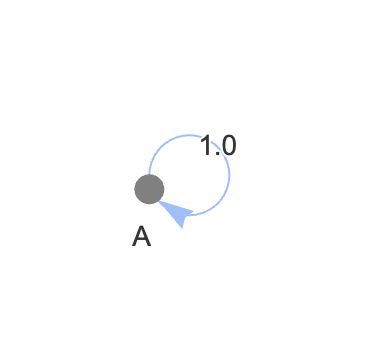
\includegraphics[width=\textwidth]{invalid_graph_1}
    \end{subfigure}
    \hfill
    \begin{subfigure}[t]{0.32\textwidth}
        \centering
        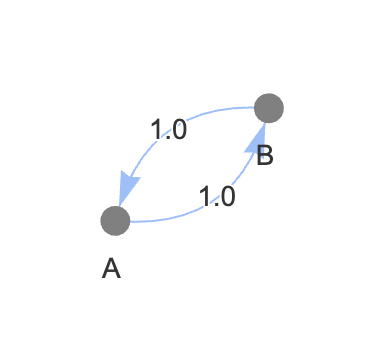
\includegraphics[width=\textwidth]{invalid_graph_2}
    \end{subfigure}
    \hfill
    \begin{subfigure}[t]{0.32\textwidth}
        \centering
        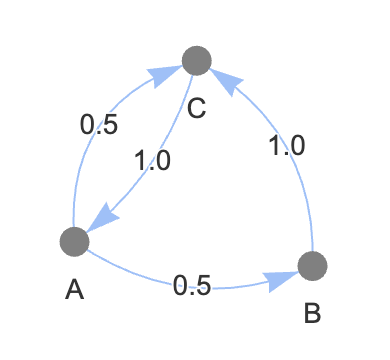
\includegraphics[width=\textwidth]{invalid_graph_3}
    \end{subfigure}
    \caption{Closed delegation cycles}
    \label{fig:closed-delegation-cycles}
\end{figure}

\Cref{fig:closed-delegation-cycles} shows exemplary closed delegation cycles. These cycles lead to contradictory situations, as power delegated within never reaches a sink. Some works discuss ways to handle power stuck in such cycles or mitigate the risk of such cycles appearing, but effectively it is lost. \cite{behrensCircularDelegationsMyth2015, brillInteractiveDemocracy2018} This means that none of the nodes in a closed cycle will vote, which is in line with the will of voters, who all wish to not vote themselves, instead delegate their power, letting their delegate(s) decide what to do with this power. 

In practice, such cycles need to be addressed before resolving delegations in a preprocessing step. Our approach to this is to find all such cycles, and collapse them into an additional sink node in the graph, the \textbf{cycle sink node}. Any delegation into the cycle is redirected into the cycle sink node,  thus ensuring the graph no longer has any closed delegation cycles. The algorithm to do so can be found in annex XX. \TODO{Add this into the annex, if that necessary...} 

We prove below, that given the absence of such closed delegation cycles, delegations are resolvable given a delegation graph. 

\begin{theorem}
Let $G = (S \dot\bigcup D, E)$ be a delegation graph. If $G$ contains no closed delegation cycles, then for every delegator $d \in D$, there exists a path from $d$ to a sink node $s \in S$.
\end{theorem}
\begin{proof}
Suppose, for contradiction, that $G$ contains no closed delegation cycle, but $\exists d \in D$ such that no path from $d$ leads to any sink $s \in S$. Since G is a finite graph, any walk from $d$ must eventually repeat nodes, implying a cycle. If at least one node in this cycle can reach a sink, there would be a path for all others in the cycle to reach a sink via this node as well, thus all nodes in the cycle can not reach a sink either. Thus, G does contain a closed delegation cycle. $\lightning$
\end{proof}

We define a \textbf{well-formed delegation graph} as a delegation graph, which contains no closed delegation cycles. Note, that while a self loop of weight one is not allowed in a well-formed delegation graph, a self loop of weight $w < 1$ is allowed as long as the rest of the node's power eventually flows to a sink. Since a delegator cannot vote themselves, any power it delegates to itself will "flow" back into the node, and then be redistributed to its delegates. 

\section{Resolving Delegations}
\label{sec:resolving_delegations}

\begin{figure}[t]
	\centering
	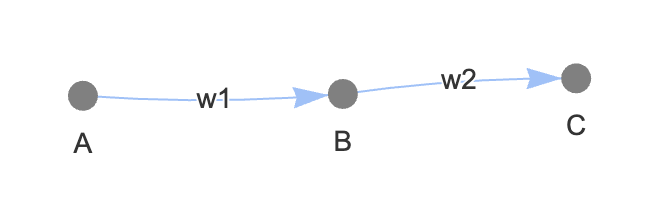
\includegraphics[width=0.4\textwidth]{delegation_graph_sample}
	\caption{Sample delegations}
	\label{fig:sample_delegations}
\end{figure}

We will use the sample delegation chain in \cref{fig:sample_delegations} to create an intuition on how we will resolve delegation graphs. Sink node $C$ receives its own initial vote, and is also delegated a fraction $w_2$ of $B$'s vote. Node $B$, in turn, receives its own vote and a fraction $w_1$ of A's vote. Let $p'_A$ and$ p'_B$ denote the \textbf{standing power} of nodes $A$ and $B$, i.e. the total amount of power delegated to them. Then, the final power of $C$, assuming no other incoming delegations, is:

\begin{align*}
p_C &= 1 + w_2p'_B \\
&= 1 + w_2(1 + w_1p'_A) \\
&= 1 + w_2(1 + w_1 \cdot 1)
\end{align*}

This motivates the recursive definition of standing power in a delegation graph $G = (V, E)$ as:

\[
p'_v = 1 + \sum_{(u, v, w) \in E} wp'_u
\]

Using this definition, and in line with the problem statement that delegating nodes must not retain any power, we define the final voting power $p_v$ of a node as:
\[
p_v = 
\begin{cases}
p'_v & \text{if } v \in S \\
0     & \text{if } v \in D
\end{cases}
\]

The problem of finding each node's standing power is thus a problem of solving a system of linear equations, namely calculating the standing power for all nodes. We can prove, that given a well-formed delegation graph, this method returns a unique solution, and power is conserved.

\subsection{Existence of a Unique Solution}
\label{subsec:unique_sol}

The system of linear equations $p'_v = 1 + \sum_{(u, v, w) \in E} wp'_u$ can also be rearranged to be in matrix form: 

\begin{align*}
p' = \mathbb{1} + Wp' &\implies p' - Wp' = \mathbb{1} \\
&\implies (I - W)p' = \mathbb{1}
\end{align*}

where \( p' \in \mathbb{R}_+^{|V|} \) is the vector of standing power values for each node, \( W \in (0, 1]^{|V| \times |V|} \) is the adjacency matrix of the graph (with \( W_{ij} \) denoting the weight of the edge from node \( j \) to node \( i \)), and \( \mathbb{1} \) is the all-ones vector. This notation will be used within the proof below.

\begin{theorem}
Given a well-formed delegation graph $G=(V, E)$, the equation $p'_v = 1 + \sum_{(u, v, w) \in E} wp'_u$ has a unique solution for all $v \in V$.
\end{theorem}
\begin{proof}

The theorem holds trivially if $|V| = 0$, since the statement “for all $v \in V$” is vacuously true.

Assume now that $G = (V, E)$ contains at least one node. Let $G' = (V, E')$, where
\[
E' = E \cup \{(s, s, 1) \mid s \text{ is a sink in } V\}.
\]
By construction, each node in $G'$ has outgoing edges whose weights sum to 1, so $G'$ is a (row-stochastic) Markov chain. Furthermore, $G$ satisfies the following:

\begin{enumerate}
\item There exists at least one sink (follows from well-formedness and $|V| > 0$),
\item Every node has a path to at least one sink (by assumption on well-formed delegation graphs).
\end{enumerate}

Thus, $G'$ is an absorbing Markov chain: every state can reach an absorbing state (a sink with a self loop) in finite steps. A standard result for such chains is that their transition matrix $P$ can be rearranged as:

\[
P = \begin{bmatrix}
Q & R \\
0 & I_r
\end{bmatrix},
\]

where $Q$ describes transitions between transient (non-sink) states, $R$ transitions from transient to absorbing states, and $I_r$, the identity matrix, the transitions from absorbing states, which necessarily always transition back into themselves. After infinite transitions, the probability of still being in a transient state is zero, thus $\lim_{k \to \infty} Q^k = 0$, which implies that $Q$'s spectral radius $\rho(Q) < 1$.

Now consider the system of linear equations

\[
(I - W)p' = \mathbb{1}
\]

Let $W^T$ be $W$'s transpose. Then $W^T$ structurally resembles a transition matrix, with row sums = 1.

Define the subgraph $D \subset G$ induced by all delegating (non-sink) nodes. Let $W_D^T$ be the transpose of the weight matrix for $D$, which only includes delegations among delegating nodes. 

Then $W_D^T = Q$, so $W_D = Q^T$ and $\rho(W_D) = \rho(Q) < 1$. The equality of the two matrices follows from the observation that the construction of $G'$ from $G$ only adds self-loops to sink nodes, leaving all delegating nodes and their outgoing edges unchanged.

Note that standing power values for delegating nodes depend only on the values of other delegators — never on sink nodes. This justifies restricting the analysis to the submatrix $W_D$, as the equation system governing these nodes is self-contained.

We now restrict our attention to the system of equations over only the transient nodes:
\[
(I - W_D) p'_D = \mathbb{1}.
\]

Since $\rho(W_D) < 1$, the Neumann series
\[
(I - W_D)^{-1} = \sum_{k=0}^{\infty} W_D^k
\]
converges, and thus $(I - W_D)$ is invertible. Therefore, $p'_D$ has a unique solution.

Finally, since the standing power of each sink depends only on the standing power values of delegators, and those are uniquely determined, the full vector $p'$ is uniquely determined as well.
\end{proof}

 \subsection{Conservation of Power}
 
 In order to assure that the power is conserved during delegation, it may seem intuitive to add a constraint $\sum_{s \in S} p_s = |V|$ to the system of linear equations. However, we prove that such an equation is not necessary, as the other equations in the system of equations already imply the conservation of power.

We start with the solutions $\{p'_v | v \in V\}$.

Summing over all $v \in V$:
\begin{align*}
\sum_{v \in V} p'v &= \sum_{v \in V} \left( 1 + \sum_{(u, v, w) \in E} wp'_u \right) \\
&= |V| + \sum_{(u, v, w) \in E} wp'_u \numberthis \label{eq:cons_1}
\end{align*}

Now regroup the second term by the source node $u$:

\begin{align*}
\sum_{(u, v, w) \in E} wp'_u &= \sum_{u \in V} \sum_{(u, v, w) \in E} wp'_u  \\ 
&= \sum_{u \in V} p'_u  \sum_{(u, v, w) \in E} w \\
\intertext{
According to our definition of a delegation graph, all sinks have no outgoing notes, and all delegators's outgoing node weights add up to 1. So, for any node $u$::
\[
\sum_{(u, v, w) \in E} w = \begin{cases} 1, u \in D \\ 0, u \in S \end{cases}
\]
Thus we can split the outer sum:
} 
&= \left(\sum_{u \in D} p'_u  \sum_{(u, v, w) \in E} w \right) + \left( \sum_{u \in S} p'_u  \sum_{(u, v, w) \in E} w \right) \\
&= \left( \sum_{u \in D} p'_u \cdot 1 \right) + \left(\sum_{u \in S} p'_u \cdot 0 \right) \\
&= \sum_{u \in D} p'_u \numberthis \label{eq:cons_2}
\end{align*}


At the same time, $V = S \bigcup D$ , and $S$ and $D$ are disjunct, we can split the term $\sum_{v \in V} p'_v$ into:

\[
\sum_{v \in V} p'_v = \sum_{v \in S} p'_v  + \sum_{v \in D} p'_v \numberthis \label{eq:cons_3}
\]

Therefore, combining \eqref{eq:cons_2} and \eqref{eq:cons_3}, the original equality \eqref{eq:cons_1} turns into:

\begin{align*}
\sum_{v \in S} p'_v  + \sum_{v \in D} p'_v &= |V| + \sum_{u \in D} p'_u \\
\implies \sum_{v \in S} p'_v  &= |V| \qed
\end{align*}

\subsection{Resolving Delegations by Solving a System of Linear Equations}

With the insights gained in the previous sections in mind, it is now possible to formulate the following method to resolving delegation graphs.

\begin{enumerate}
\item Set up a system of linear equations, such that for each node $v \in V$ there is an equation $p'_v = 1+\sum_{(u, v, w) \in E}wp'_u$
\item Solve the system of linear equations to find the value of $p'_v$ for all $v \in V$
\item For each $s \in S$ set $p_s = p'_s$
\item For each $d \in D$ set $p_d = 0$
\end{enumerate}

